\section{Basic Background in Deep Learning\label{sec:background_nn}}
In this section, we recall some basic background in \textit{deep learning}. For further detail on NN architectures see, \eg, \cite{tuto-lstm:2019:staudemeyer}.

\subsection{Neural Networks\label{sec:nn}}
\textit{Neural networks} (NNs) are a class of statistical connectionist models trained using the \textit{backpropagation} algorithm.
The training is done by processing inputs with the model and evaluating the quality of the output using a \textit{loss function}.
By minimizing this loss with an optimization algorithm, the model learns to approximate the expected output.
In this subsection, we detail several kinds of model designs (or \textit{architectures}) frequently used in deep learning.

%For detailed information on the neural architectures mentioned in this paragraph, we recommend~\cite{tuto-lstm:2019:staudemeyer}.
A multi-layer perceptron (MLP) is the simplest architecture of NN.
It is composed of multiple layers, called \textit{feed-forward layers}.
Each output of a feed-forward layer is a linear composition of all the layer's inputs.
Between layers, the values are transformed by an \textit{activation function} to increase the expressive capacity of the model.
The \textit{rectified linear unit} (ReLU) and \textit{sigmoid} are among the most common activation functions.
\cref{fig:basic-nn-architectures} contains a simple diagram of the MLP.

\begin{figure}
    \centering
    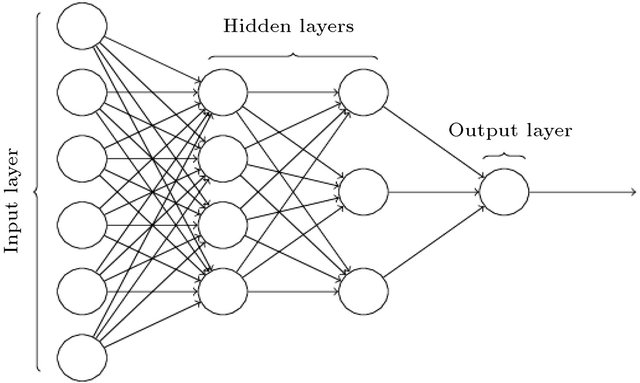
\includegraphics[keepaspectratio, width=.9\textwidth, height=5cm]{Figures/Ch0/mlp}
    \caption{Multi-layer perceptron architecture. From \footnotesize{\url{https://www.researchgate.net/profile/Ayhan_Erdem2/publication/319309006}}.}
    \label{fig:basic-nn-architectures}
\end{figure}

\subsection{Deep Learning Algorithms}
To train NNs we use specific algorithms called \textit{optimizers} to update the \textit{parameters} of the NN model based on the value of a loss function.
The parameters are the numerical values involved in the NN computations.% In the case of an MLP, the parameters are the coefficients of the linear composition functions of all the neurons of all the layers.

Training is performed by iteratively updating the \textit{parameters} of the NN, by presenting it with \textit{batches} (groups) of input samples and applying the optimizer based on the loss.
An \textit{epoch} is when all the data available is processed once.
The process is usually repeated for multiple epochs until the model \textit{converges}, in other words, until the performance of the model stops improving.

There exist a variety of optimizers, but the most recommended one~\cite{optim:2016:ruder} currently is Adam~\cite{adam:2015:kingma}.
For an overview of existing optimizers see, \eg, \cite{optim:2016:ruder}.
In our experiments, we use Adam.
This particular algorithm has low computational and memory usage compared to other algorithms and is well suited for complex optimization problems.

\subsection{Usual Loss Functions}
The loss function to use depends on the kind of problems handled.
%
When predicting specific values within a set of known values, it is standard to make the NN output probabilities of being in each of the possible values.
Typical examples are classification problems and language modeling, where the model has to predict the most likely character or word among known ones.
For those problems, we usually use the \textit{cross-entropy} loss to make the predicted probabilities closer to the actual ones.
In the binary case (only 2 possible values), we use the \textit{binary cross-entropy} (BCE) which only requires the probabilities of one of the two classes. \cref{equ:ce} is the equation of the cross-entropy with $X$ the set of all possible values, $p$ the target distribution, $q$ the predicted distribution, and $p(x)$ (or $q(x)$) the probability to have the value $x$ according to $p$ (respectively $q$). \cref{equ:bce} is the equation of the BCE with two values $0$ and $1$, but computed only using $1$.
%
Another common kind of problem is predicting real-valued data or integers, \eg, image generation.
In those cases, we typically use \textit{mean squared error} (MSE) to reduce the squared distance between the predicted value and the expected one.
\cref{equ:mse} is the equation of the MSE with $p$ and $q$ the target and the prediction.
%
Other loss functions are widespread, \eg, the cosine similarity, but we mainly use cross-entropy, BCE, MSE, and loss functions derived from those three.

\begin{align}
    H(p, q) =& - \sum_{x\in X} p(x) log(q(x)) \label{equ:ce}\\
    BCE(p, q) =& - p(1) \times log(q(1)) - (1-p(1)) \times log(1-q(1))\label{equ:bce}\\
    MSE(p, q) =& \sum_{i = 1}^{|p|}(p_i - q_i)^2\label{equ:mse}
\end{align}

\subsection{Binary Encoding and Softmax}
In classification problems the possible values are usually indexed, and a specific label is represented by a binary vector.
We speak of the \textit{binary encoding} of a set of values and \textit{one-hot encoding} of a value. Those encodings are computed with regards to the indexed set of all possible values.
In our setup, the binary encoding of a set of attributes $X \subseteq A$ is the vector of size $|A|$, such that the position $k$ of the vector contains $1$ if $a_k\in X$ and $0$ otherwise. The one-hot encoding of an attribute $a_k$ is the binary encoding of $\{a_k\}$, in other words the vector of size $|O|$ full of $0$ except at position $k$ which is $1$.

When performing a single-label classification, we usually generates the probablility for each value to be the correct one.
To obtain this set of probabilities we usually use the \textit{softmax} function, which transforms any finite set of numbers into a probability distribution.
In other words, it transforms the values into probabilities (between 0 and 1) in such a way that the sum of all values is equal to 1 and that the proportions between the values are preserved.

%In this section, we use the notions of \textit{binary} encoding of a set and \textit{one-hot} encoding of an element. Those encoding are computed with regards to the indexed set of all possible values.

%In this section we introduce the \textit{softmax} function, which transforms any finite set of numbers into a probability distribution.
%In other words, it transforms the values into probabilities (between 0 and 1) in such a way that the sum of all values is equal to 1 and that the proportions between the values are preserved.

\subsection{Major Neural Networks Architectures}
A \textit{convolutional neural network} (CNN) is a NN that apply \textit{convolutions} on an input. For an overview of CNN see, \eg, \cite{cnn-overview:2018:yamashita}.
Following the principle of \textit{convolutions}, for a given input element, a CNN produces an output based on a learned \textit{kernel} and the neighborhood of the input. It is possible to compute the size of the output and the size of the neighborhood taken into account by the CNN.
A CNN can handle inputs of varying sizes, and the output size is proportional to the ones of the input.
Additionally, CNNs maintain the relations between neighboring elements and is invariant to translation.
In other words, a CNN will produce the same output for a given neighborhood at different locations in the input.
They are widely used in image processing due to this property allowing it to learn filters to detect features independently of the position in the input.
A basic CNN is shown in \cref{fig:nn-architectures-cnn}.

\begin{figure}
    \centering
    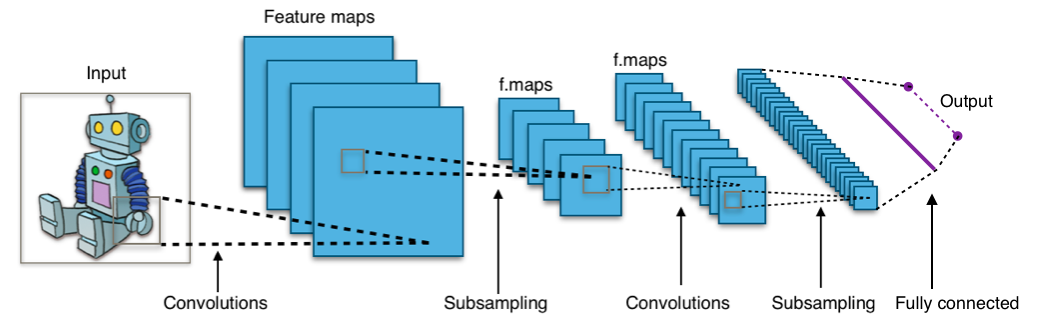
\includegraphics[keepaspectratio, width=.9\textwidth, height=5cm]{Figures/Ch0/cnn.png}
    \caption{Example of CNN architecture. From Wikipedia.}
    \label{fig:nn-architectures-cnn}
\end{figure}

The famous \textit{long short-term memory recurrent NN} (LSTM)~\cite{blstm:2005:graves} and \textit{gated recurrent unit NN} (GRU)~\cite{gru:2014:cho} are architectures of a family called \textit{recurrent NNs} (RNNs).
This family of models handles sequences of inputs of variable length, and are designed to learn dependencies within the input sequence.
By transmitting and updating a vector called \textit{hidden state} from one step of the sequence to the following one, each output depends on the current input as well as the previous ones.
A variant of the LSTM, called \textit{bi-directional LSTM} (BLSTM)~\cite{blstm:2005:graves}, uses a second LSTM to process the input sequence in the reverse direction. It can thus handle both forward and backward dependencies in the sequence.
A major flaw of all RNNs is their inability to model long-range dependencies, with various variants like LSTM and GRU trying to solve this \textit{memory} issue to some extent.
A block diagram representing how RNN handle sequences is shown in \cref{fig:nn-architectures-rnn-unfolded}, and the inner workings of a a GRU and an LSTM are shown respectively in \cref{fig:nn-architectures-gru}, and \cref{fig:nn-architectures-lstm}.

\begin{figure}
    \centering
    \subcaptionbox{RNN\label{fig:nn-architectures-rnn-unfolded}}{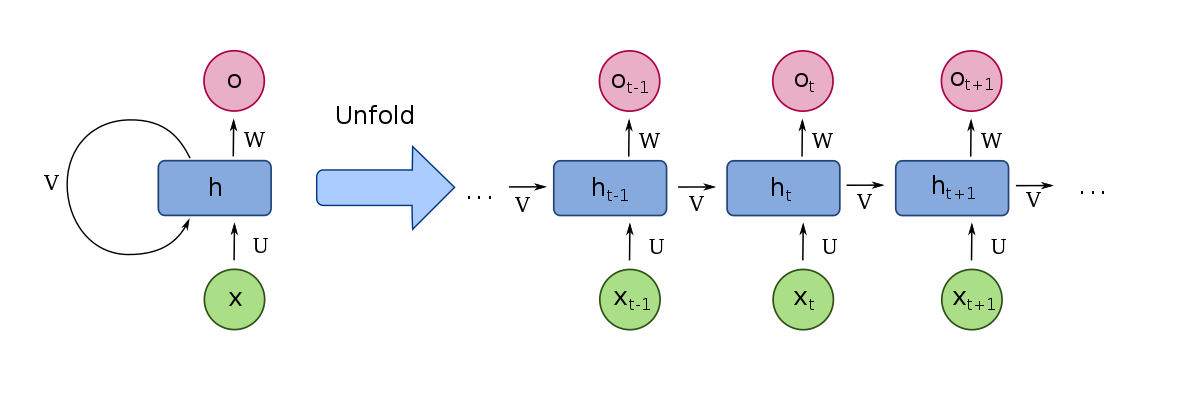
\includegraphics[keepaspectratio, width=.9\textwidth, height=4cm]{Figures/Ch0/rnn.png}}
    \subcaptionbox{GRU cell\label{fig:nn-architectures-gru}}{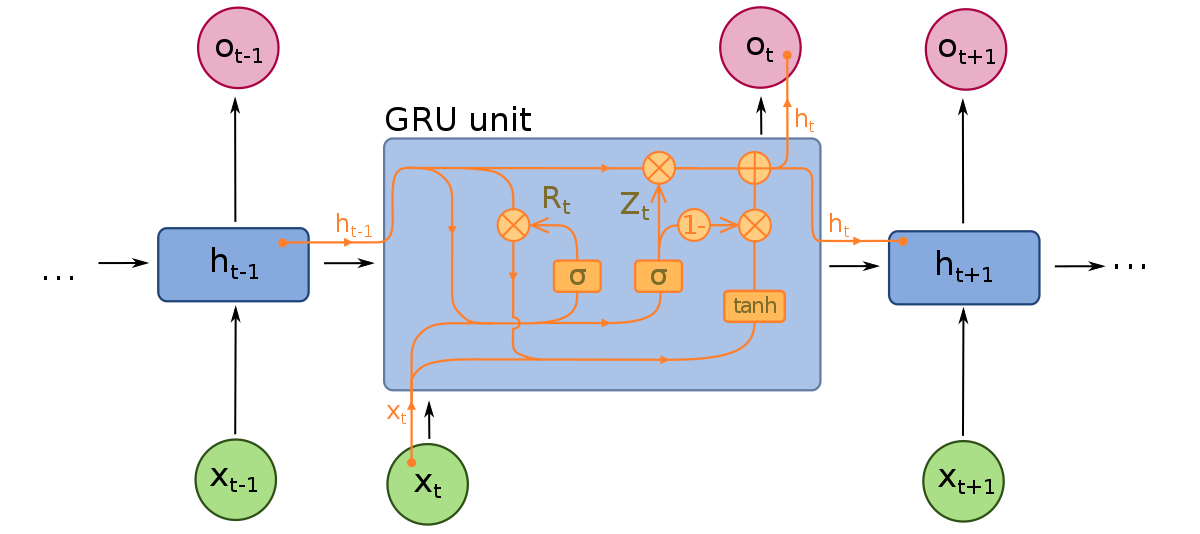
\includegraphics[keepaspectratio, width=.48\textwidth, height=5cm]{Figures/Ch0/gru_cell.png}}
    \subcaptionbox{LSTM cell\label{fig:nn-architectures-lstm}}{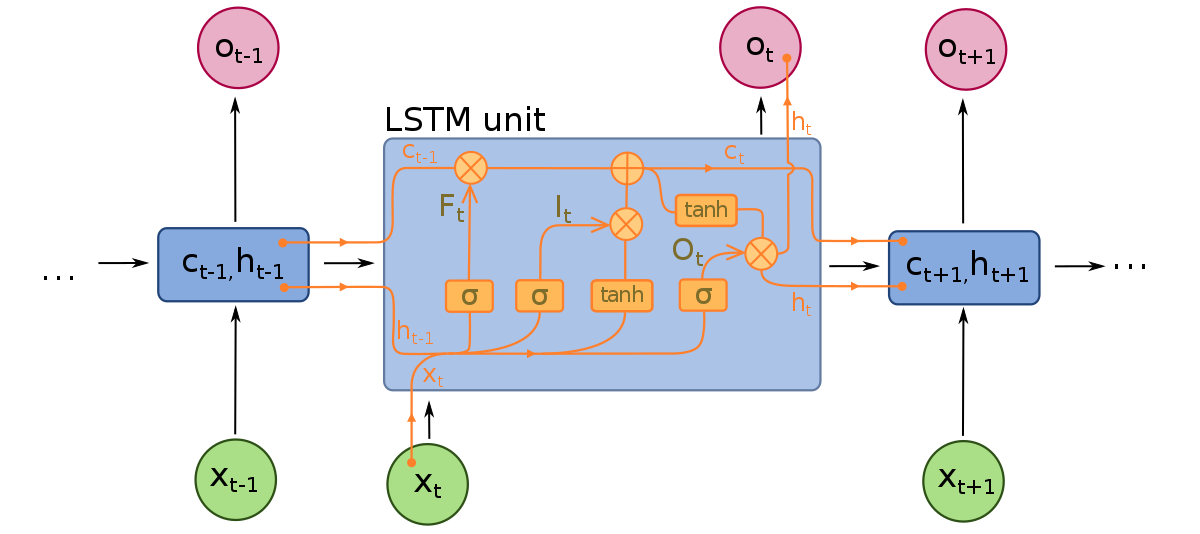
\includegraphics[keepaspectratio, width=.48\textwidth, height=5cm]{Figures/Ch0/lstm_cell.png}}
    \label{fig:nn-architectures-rnns}
    \caption{Structure of the major RNN architectures, the input at step $t$ is $x_t$, the hidden state $h_t$, and the output $o_t$. From Wikipedia.}
\end{figure}

\textit{Attention} mechanisms~\cite{attention:2015:bahdanau}, which have been developed to handle this issue, consider a full sequence and attribute \textit{attention weights} to each element. The attention weights are usually computed with a \textit{dot product} between a \textit{query} and the elements in the sequence, though there are numerous variants of attention. The attention weights are usually used to weight the sequence directly or to compute a weighted average of the sequence.
The summaries produced by the attention mechanisms are called \textit{context}.
Attention is cheap to compute (usually), and the analysis of the attention weights allows to determine the implication of each element in the final result.
Due to this property, attention can be used to make an RNN's result interpretable.
Attention is powerful enough to be used alone, like the \textit{transformer network}~\cite{transformer:2017:vaswani} and more recently the \textit{reformer network}~\cite{reformer:2020:kitaev}.
An example of attention for neural machine translation is shown in \cref{fig:nn-architectures-attention}.

\begin{figure}
    \centering
    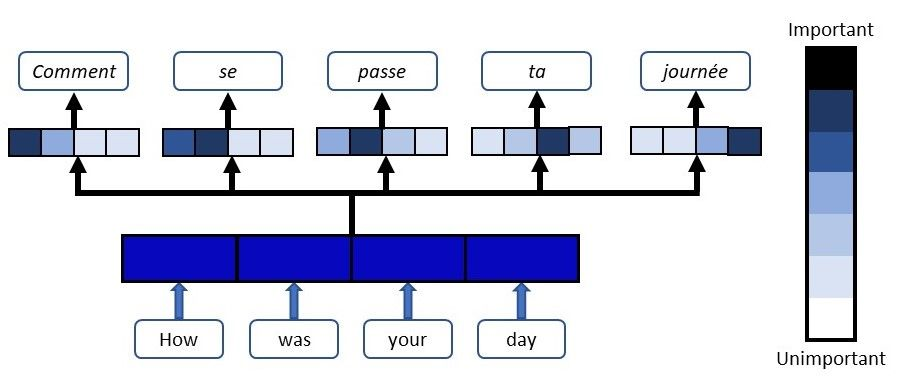
\includegraphics[keepaspectratio, width=.9\textwidth, height=5cm]{Figures/Ch0/attention.jpg}
    \caption{Example of attention mechanism for translation from English to French. From \footnotesize{\url{https://blog.floydhub.com/attention-mechanism/}}}
    \label{fig:nn-architectures-attention}
\end{figure}

We call \textit{unordered composition functions} operations that do not take into account the order of the input elements and can accommodate any number of input elements. Typical examples for vectors are the element-wise min, max, and average (also respectively called min-, max-, and average-pooling).
Unordered composition-based models combining an unordered composition of the inputs with an MLP are called \textit{deep averaging networks} (DANs).
They have proven their effectiveness in a variety of tasks, for instance, sentence embedding~\cite{dan:2015:iyyer}, sentiment classification~\cite{adan:2016:chen}, and feature classification~\cite{cdan:2017:gardner}.
On the one hand, this family of architectures allows for varying sizes of input to be processed at a relatively low computational cost, by opposition to recurrent models like LSTM.
On the other hand, the information related to the order of the input elements is lost.
The DAN for sentence embedding from~\cite{dan:2015:iyyer} is shown in \cref{fig:nn-architectures-dan}.

\begin{figure}
    \centering
    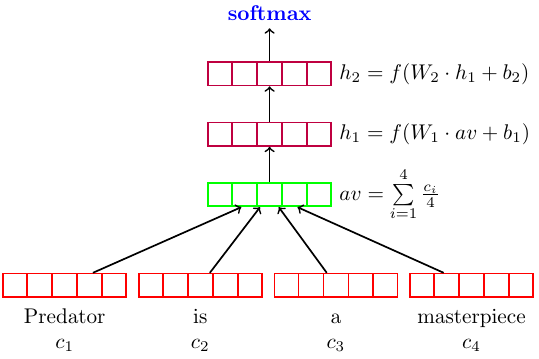
\includegraphics[keepaspectratio, width=.9\textwidth, height=5cm]{Figures/Ch0/dan.png}
    \caption{Example of DAN, Figure 1 from~\cite{dan:2015:iyyer}.}
    \label{fig:nn-architectures-dan}
\end{figure}

To summarize, CNNs, RNNs, attention mechanisms, and DANs are various architectures able to handle inputs of varying sizes, each with their advantages and drawbacks.

\subsection{Auto-Encoders and Embeddings\label{sec:vae}}
\textit{Auto-encoders} are a class of deep learning models composed of:
\textit{(i)} an encoder, taking some $x$ as an input and producing a latent representation $z$;
\textit{(ii)} a decoder, taking $z$ as an input and reconstructing $\hat{x}$ a prediction of $x$.
%The model learns to reresent $x$ into $z$ with a the training objective
By training the model to match $x$ and $\hat{x}$, the model learns to compress $x$ into $z$. We call the training objective matching $x$ and $\hat{x}$ the \textit{reconstruction loss}.
Auto-encoders are one of the methods to generate representations of data as vectors. In that case, $z$ is called the \textit{embedding} of $x$, and the real-valued space in which $z$ is defined is called the \textit{embedding space}.

%\subsubsection{Variational Auto-Encoders}
Unlike traditional auto-encoders, \textit{variational auto-encoders} (VAEs)~\cite{vae:2013:kingma} encode a distribution for each value of $z$ instead of the value itself.
In practice, for each element of $z$, the encoder produces two values: a mean $\mu$ and standard deviation $\sigma$.
When training the model, $z$ is sampled from the normal distribution defined by $\mu$ and $\sigma$.
Finally, the distribution defined by $\mu$ and $\sigma$ is normalized by using an additional loss term called \textit{Kullback–Leibler divergence} (KL divergence).
To make this process differentiable and be able to train the model, a method called \textit{reparametrization}~\cite{vae:2013:kingma} is used.

VAEs are known to provide better generalization capabilities and are easier to use to decode arbitrary embeddings, compared to classic auto-encoders.
This property is useful for generation, as we can train a model generating embeddings then decode them with a pre-trained VAE.
A typical example of VAE, is one trained on basic geometric shapes (circles, triangles, rectangles, \etc), allows us to decode arbitrary embeddings:
the average of the embedding of a triangle and a rectangle would give us a trapezoid (a coherent mix of a triangle and a rectangle) even if none were seen during training.
Thus, VAEs have been used in a wide variety of applications to improve the quality of embedding spaces: image~\cite{vae:2013:kingma}, speech~\cite{deep-metric-multispeaker:2020:kulkarni}, and graph generation~\cite{graph-vae:2016:kipf} for example.
%However, using a VAE instead of a classical auto-encoder can decrease the performance for some tasks.\todo{add citation}
%To use a VAE as an encoder once it is trained, we do not sample $z$ from the distribution and use $\mu$ .
% \begin{figure}
%     \centering
%     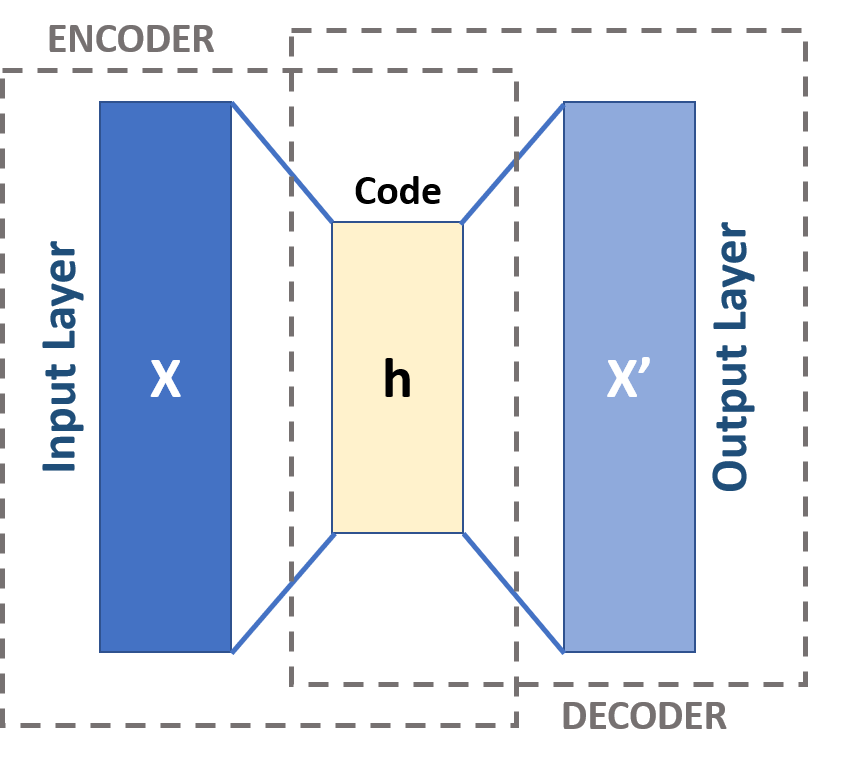
\includegraphics[keepaspectratio, width=.9\textwidth, height=5cm]{autoencoder_wiki}
%     \caption{Diagram of a basic auto-encoder. From \url{https://en.wikipedia.org/wiki/Autoencoder}.}
%     \label{fig:my_label}
% \end{figure}


A constrained VAE is a kind of VAE that feeds a \textit{constraint} vector (or \textit{condition}) to the decoder in addition to the embedding.
Because the condition already contains part of the information, the model will learn to encode the rest in the embedding.
This architecture allows to voluntarily exclude part of the information form the embedding or to constrain the decoding process.
An example of constrained VAE is~\cite{deep-metric-multispeaker:2020:kulkarni}, which uses the condition to specify the speaker in emotional speech.
The embedding contains ``anonymized'' speech information, and it becomes possible to transfer emotional speech from one speaker to another by changing the condition.

\subsection{Metric Learning}
\textit{Metric learning}~\cite{vae-metric-learning:2018:xudong} is a process used to train embedding models, by making their embedding space have properties of a metric.
To achieve this, a loss is used to reduce the distance between the embeddings of equal elements and increase the distance between embeddings of different elements.
Multiple losses can achieve this, such as \textit{pairwise loss} and \textit{triplet loss}. 
Those losses consider the embeddings of three elements: an input $x$, some $x'$ judged equal to $x$, and some $y$ different from $x$.
They are used to minimize the distance between equal elements and maximize the distance between different elements.
In some approaches~\cite{deep-metric-multispeaker:2020:kulkarni}, a predictor (typically an MLP) is used to predict a distance between the embeddings, instead of applying a standard distance directly on the embeddings.

It is possible to learn metrics on different aspects of the elements, by splitting the embedding into different segments and learn a different metric on each segment~\cite{deep-metric-multispeaker:2020:kulkarni}.

Metric learning is usually used to approximate actual metrics.
However, its process can be applied to learn other kinds of measures not fitting the definition of a metric.
The current paper falls in this case.